\documentclass{article}
\usepackage[utf8]{inputenc}
\usepackage[hidelinks]{hyperref}
\usepackage{color}
\usepackage{graphics}
\usepackage{graphicx}
\usepackage{amsfonts}

\usepackage[spanish]{babel}

\title{Matemáticas Computacionales \\ Practica 1: Gráficas de curvas en R}
\author{1860560 Rangel Delgado Jesus Angel}
\date{16 de Febrero del 2021}

\begin{document}

\maketitle

\section{Introducción}
\subsection{Desarrollo de la practica}
En esta primera práctica se hará una de las cosas básicas al momento de aprender R. Se repasaran las curvas en $\mathbb{R}^2$
 vistas en primer semestre en la materia de Geometría Analítica. [1].
Se graficarán curvas como la recta, parábola, circunferencia, elipse e hipérbola.

\section{Curvas de $\mathbb{R}^2$}
\subsection{Linea Recta}
\textbf{Def.} Llamamos \textbf{linea recta} al lugar geométrico de los puntos tales que tomados dos puntos diferentes cualesquiera $P_1$($x_1$, $y_1$) y $P_2$($x_2$, $y_2$) de lugar, el valor de m se calcula por medio de:

\begin{equation}
    m = \frac{y_1-y_2}{x_1-x_2}
\end{equation}

\textbf{Ecuación de la recta dada su pendiente y ordenada en el origen} Es la recta cuya pendiente \textbf{m} y cuya ordenada en el origen es \textbf{b}, que tiene por ecuación:

\begin{equation}
    y = mx+b
\end{equation}

\textbf{Código en R}
\newline Para poder graficar esta función, solo basta con darle valor a la pendiente \textbf{m} y su ordenada \textbf{b}, además falta establecer un limites que serán el extremo al que llegara nuestra función.

\newpage

\textbf{Ejemplo 1:}

\begin{figure}[h]
    \centering
    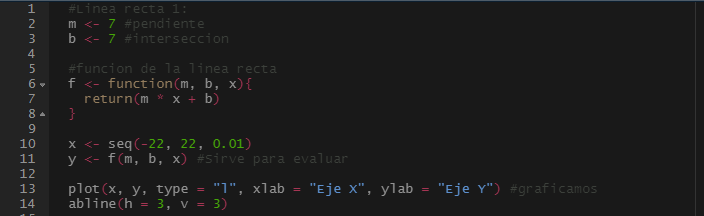
\includegraphics[width=12cm, height=5cm]{Codigolinea1}
    \caption{Código de la linea 1}
    \label{fig:mesh1}
\end{figure}
y su gráfica seria:
\begin{figure}[h]
    \centering
    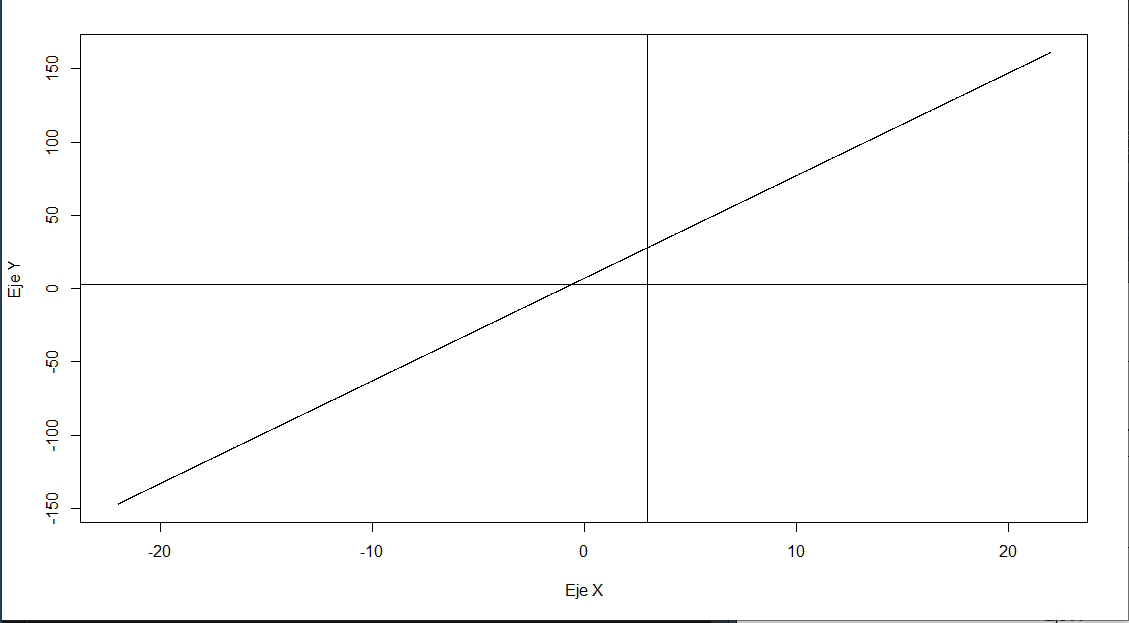
\includegraphics[width=10cm, height=5cm]{Grafica1}
    \caption{Gráfica del código 1}
    \label{fig:mesh2}
\end{figure}

\newpage

\textbf{Ejemplo 2:}

\begin{figure}[h]
    \centering
    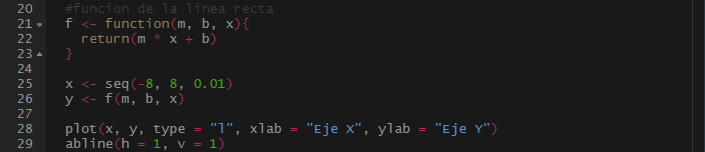
\includegraphics[width=12cm, height=5cm]{Codigolinea2}
    \caption{Código de la linea 2}
    \label{fig:mesh3}
\end{figure}
y su gráfica seria:
\begin{figure}[h]
    \centering
    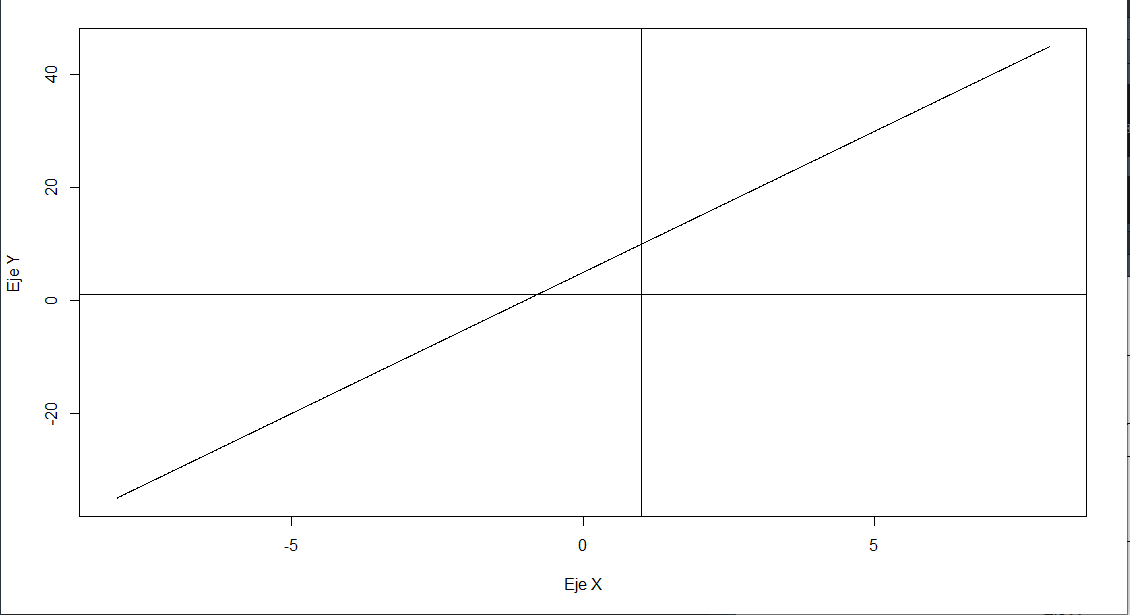
\includegraphics[width=10cm, height=5cm]{Grafica2}
    \caption{Gráfica del código 2}
    \label{fig:mesh4}
\end{figure}

\subsection{Circunferencia}
\textbf{Def.} Circunferencia es el lugar geométrico de un punto que se mueve en un plano de tal manera que se conserva siempre a una distancia constante de un punto fijo de ese plano

\textbf{Teorema}La circunferencia cuyo centro es el punto (h,k) y cuyo radio es la constante r, tiene por ecuación:

\begin{equation}
    (x-h)^2 + (y-k)^2  = r^2
\end{equation}

\newpage
\textbf{Código en R}
Para poder graficar una circunferencia en R primero tenemos que asegurarnos de que nuestra r o sea el radio de la circunferencia sea mayor que cero, después hay que comenzar a graficar por partes, nuestra circunferencia en este caso iniciamos con la parte positiva para después graficar la negativa, por ultimo se asignan valores a nuestra función, los valores para h, k y r.
\newline
\textbf{Ejemplo 1:}


\begin{figure}[h]
    \centering
    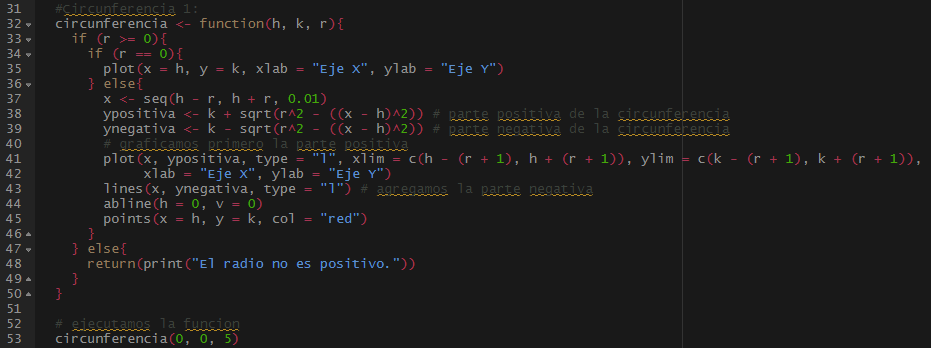
\includegraphics[width=12cm, height=5cm]{Codigocircu1}
    \caption{Código de la circunferencia 1}
    \label{fig:mesh7}
\end{figure}
y su gráfica seria:
\begin{figure}[h]
    \centering
    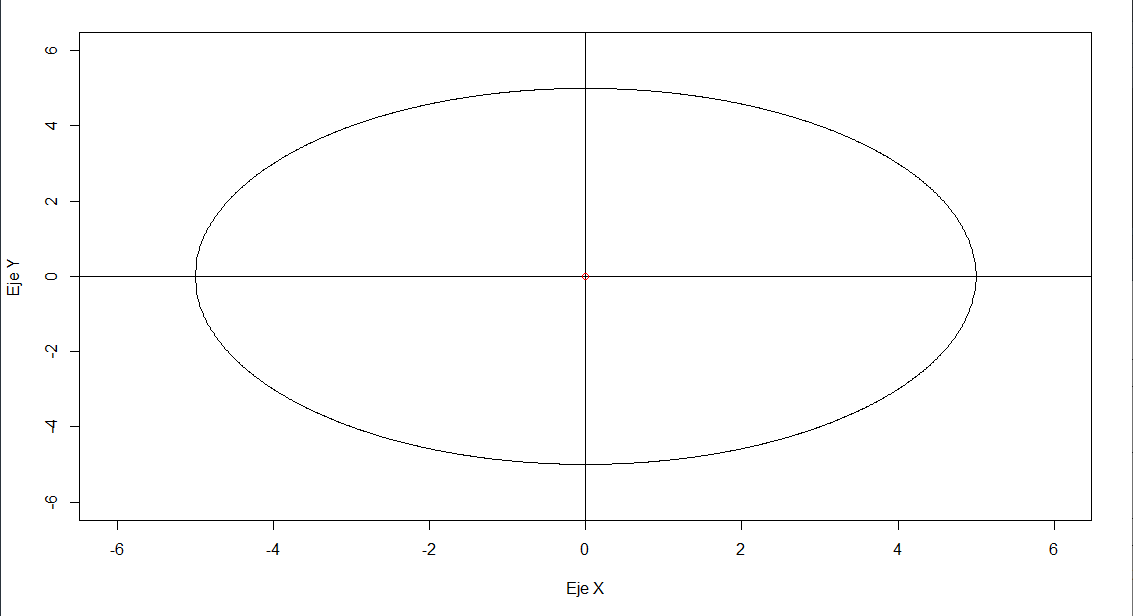
\includegraphics[width=10cm, height=5cm]{Grafica3}
    \caption{Gráfica de la circunferencia 1}
    \label{fig:mesh8}
\end{figure}

\newpage

\textbf{Ejemplo 2:}


\begin{figure}[h]
    \centering
    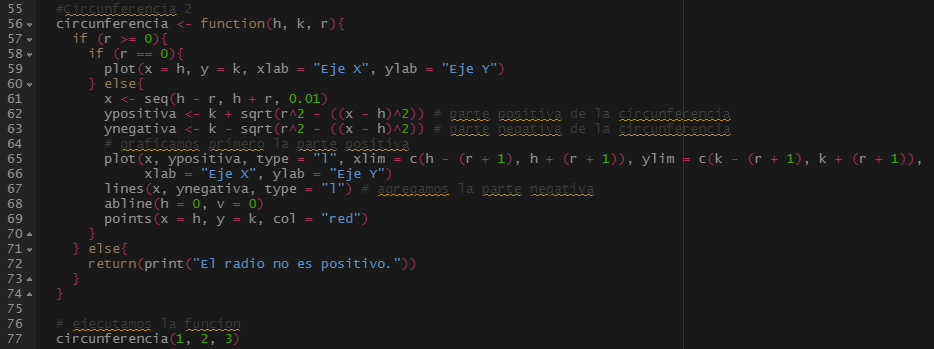
\includegraphics[width=12cm, height=5cm]{Codigocircu2}
    \caption{Código de la circunferencia 2}
    \label{fig:mesh5}
\end{figure}
y su gráfica seria:
\begin{figure}[h]
    \centering
    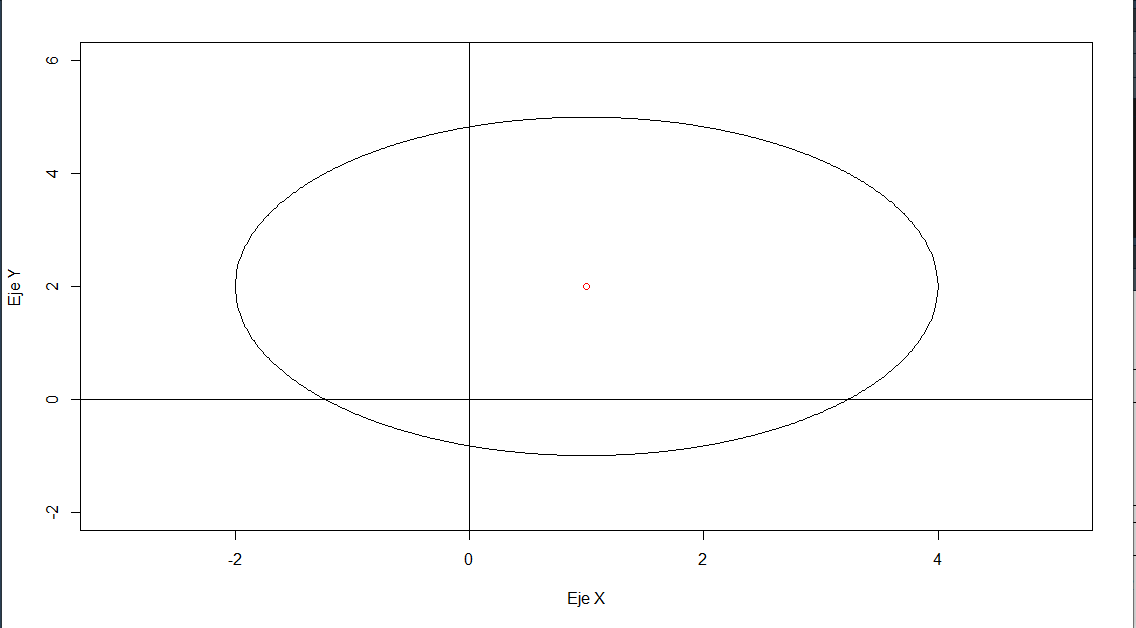
\includegraphics[width=10cm, height=5cm]{Grafica4}
    \caption{Gráfica de la circunferencia 2}
    \label{fig:mesh6}
\end{figure}



\subsection{Parábola}
\textbf{Def.} Una parábola es un lugar geométrico de un punto que se mueve en un plano de tal manera que su distancia de una recta fija, situada en el plano, es siempre igual a su distancia de un punto fijo del plano y que no pertenece a la recta.
\newline
\textbf{Las ecuaciones con vértice en el origen}
\begin{equation}
    y^2 = 4px
\end{equation}

\begin{equation}
    x^2 = 4py
\end{equation}
\newline
\textbf{Las ecuaciones con vértice fuera del origen}

\begin{equation}
    (y-k)^2 = 4p(x-h)
\end{equation}

\begin{equation}
    (x-h)^2 = 4p(y-k)
\end{equation}

\textbf{Código en R}
\newline Para poder graficar una Parábola en R, solo basta con introducir una ecuación que genere una parábola y al igual que en los casos anteriores introducir el código correspondiente para graficar.
\newline
\textbf{Ejemplo 1}

\begin{figure}[h]
    \centering
    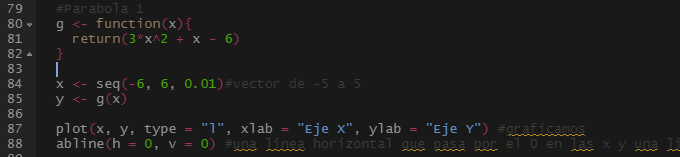
\includegraphics[width=12cm, height=5cm]{Codigopara1}
    \caption{Código de la parábola 1}
    \label{fig:mesh9}
\end{figure}
y su gráfica seria:
\begin{figure}[h]
    \centering
    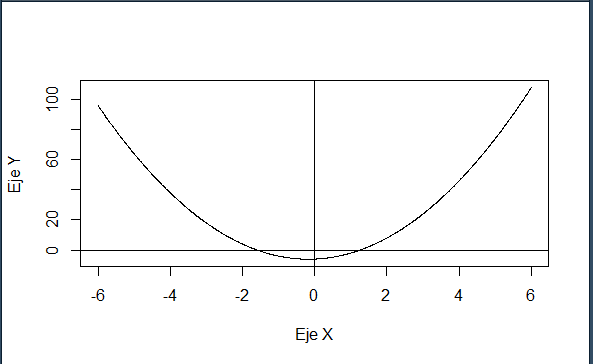
\includegraphics[width=10cm, height=5cm]{Grafica5}
    \caption{Gráfica de la parábola 1}
    \label{fig:mesh10}
\end{figure}

\newpage
\textbf{Ejemplo 2:}


\begin{figure}[h]
    \centering
    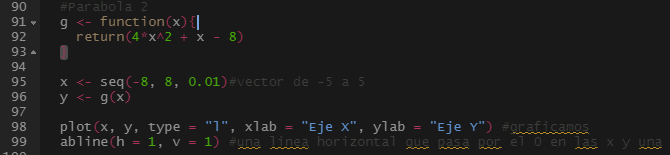
\includegraphics[width=12cm, height=5cm]{Codigopara2}
    \caption{Código de la parábola 2}
    \label{fig:mesh11}
\end{figure}
y su gráfica seria:
\begin{figure}[h]
    \centering
    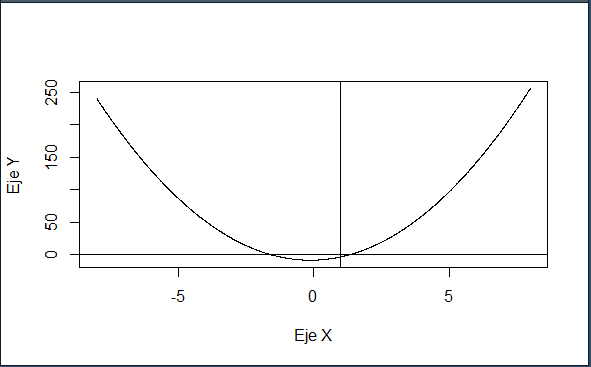
\includegraphics[width=10cm, height=5cm]{Grafica6}
    \caption{Gráfica de la parábola 2}
    \label{fig:mesh12}
\end{figure}

\subsection{Elipse}
\textbf{Def.} Una elipse es el lugar geométrico de un punto que se mueve en un plano de tal manera que la suma de sus distancias a dos fijos de ese plano es siempre igual a una constante, mayor que la distancia entre los dos puntos.
\newline
\textbf{Las ecuaciones con vértice en el origen}
\begin{equation}
    \frac{x^2}{a^2} + \frac{y^2}{b^2} = 1
\end{equation}

\begin{equation}
    \frac{x^2}{b^2} + \frac{y^2}{a^2} = 1
\end{equation}
\newline
\textbf{Las ecuaciones con vértice fuera del origen}
\begin{equation}
    \frac{(x-h)^2}{a^2} + \frac{(y-k)^2}{b^2} = 1
\end{equation}

\begin{equation}
    \frac{(x-h)^2}{b^2} + \frac{(y-k)^2}{a^2} = 1
\end{equation}

\textbf{Código en R}
\newline Para poder graficar una elipse en R, se sigue casi el mismo procedimiento que al graficar una circunferencia ya que se gráfica por partes, primero la positiva y luego la negativa, solo que a diferencia de la circunferencia esta tiene muchas condiciones a las cuales esta ligada y se tienen que cumplir.
Por ultimo solo es cuestión de asignar valores como el centro, a y b para graficar la elipse
\newline
\textbf{Ejemplo 1}

\begin{figure}[h]
    \centering
    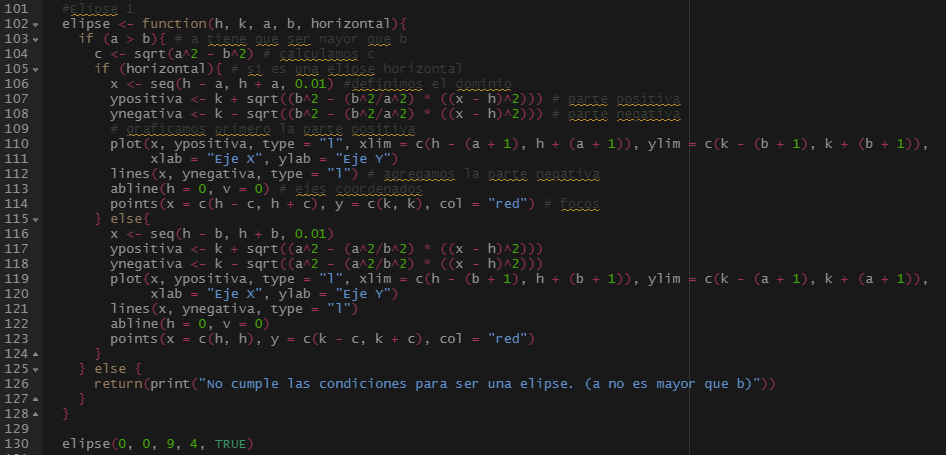
\includegraphics[width=12cm, height=5cm]{Codigoelipse1}
    \caption{Código de la elipse 1}
    \label{fig:mesh13}
\end{figure}
y su gráfica seria:
\begin{figure}[ht]
    \centering
    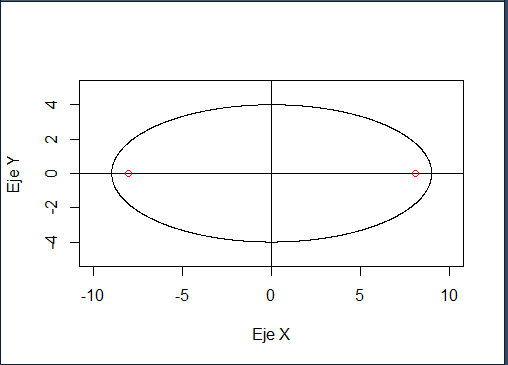
\includegraphics[width=10cm, height=5cm]{Grafica7}
    \caption{Gráfica de la elipse 1}
    \label{fig:mesh14}
\end{figure}

\newpage
\textbf{Ejemplo 2:}
\begin{figure}[h]
    \centering
    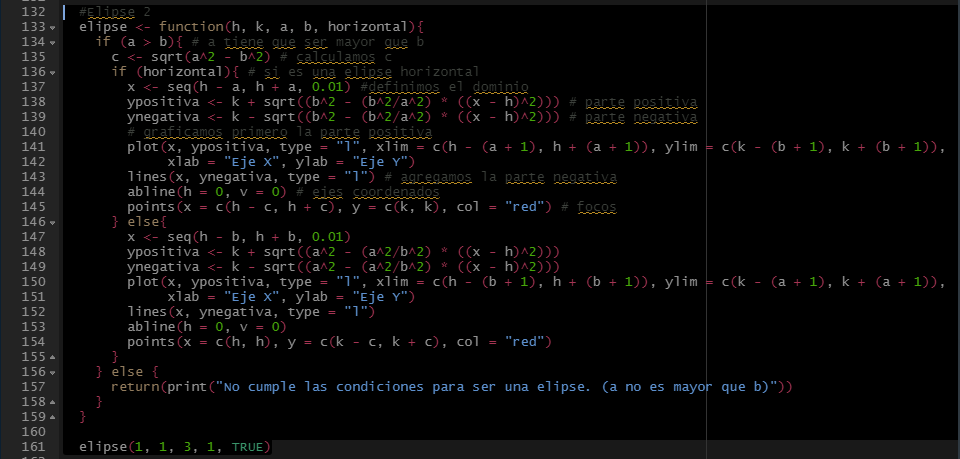
\includegraphics[width=12cm, height=5cm]{Codigoelipse2}
    \caption{Código de la elipse 2}
    \label{fig:mesh15}
\end{figure}


\newpage

y su gráfica seria:
\begin{figure}[ht]
    \centering
    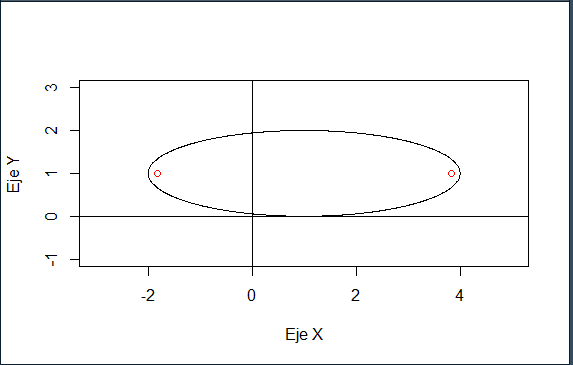
\includegraphics[width=10cm, height=5cm]{Grafica8}
    \caption{Gráfica de la elipse 2}
    \label{fig:mesh16}
\end{figure}


\subsection{Hipérbola}
\textbf{Def.} Una hipérbola es el lugar geométrico de un punto que se mueve en un plano de tal manera que el valor absoluto de la diferencia de sus distancias a dos puntos fijos del plano, llamados focos, es siempre igual a una cantidad constante, positiva y menor que la distancia entre los focos
\newline
\textbf{Ecuaciones con vértice en el origen}

\begin{equation}
    \frac{x^2}{a^2} - \frac{y^2}{b^2} = 1
\end{equation}

\begin{equation}
    \frac{x^2}{b^2} - \frac{y^2}{a^2} = 1
\end{equation}
\newline
\textbf{Ecuaciones con vértice fuera del origen}
\begin{equation}
    \frac{(x+h)^2}{a^2} - \frac{(y+k)^2}{b^2} = 1
\end{equation}

\begin{equation}
    \frac{(x+h)^2}{b^2} - \frac{(y+k)^2}{a^2} = 1
\end{equation}

\textbf{Código en R}
\newline Para poder graficar una hipérbola en R es necesario crear una función que nos ayude a descifrar como se graficara nuestra función una vez que se ingresen los valores del centro (h, k) y los valores de a y b, es importante que en la función se agregue ciertas condiciones para que se creen las hipérbolas en ambos lados.

\newpage
\textbf{Ejemplo 1:}

\begin{figure}[h]
    \centering
    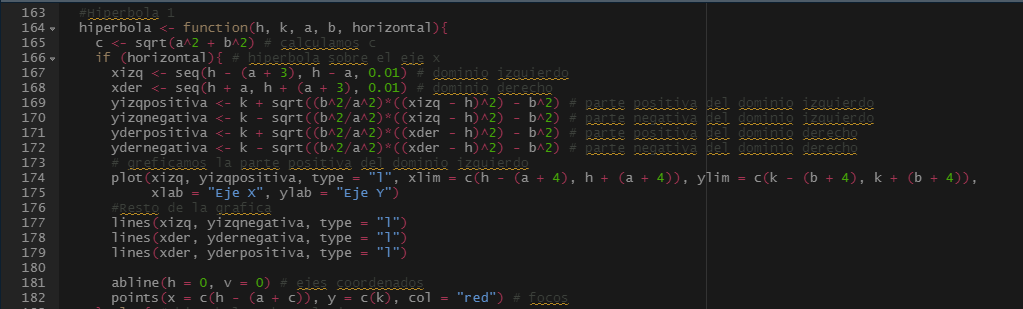
\includegraphics[width=12cm, height=5cm]{Codigohipe1}
    \caption{Código de la hipérbola 1 parte 1}
    \label{fig:mesh17}
\end{figure}
\begin{figure}[h]
    \centering
    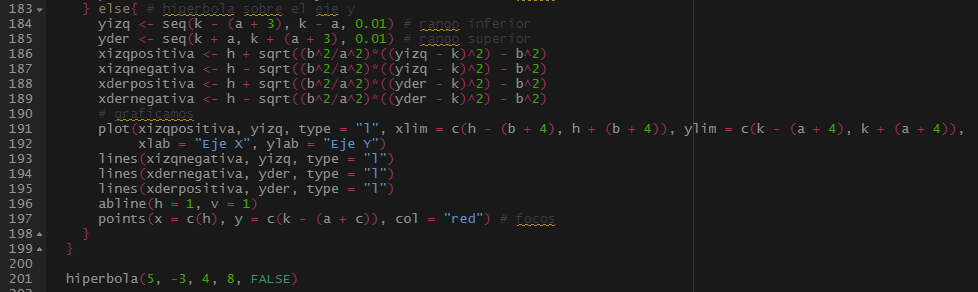
\includegraphics[width=12cm, height=5cm]{Codigohipe2}
    \caption{Código de la hipérbola 1 parte 2}
    \label{fig:mesh18}
\end{figure}
\newpage
y su gráfica seria:
\begin{figure}[ht]
    \centering
    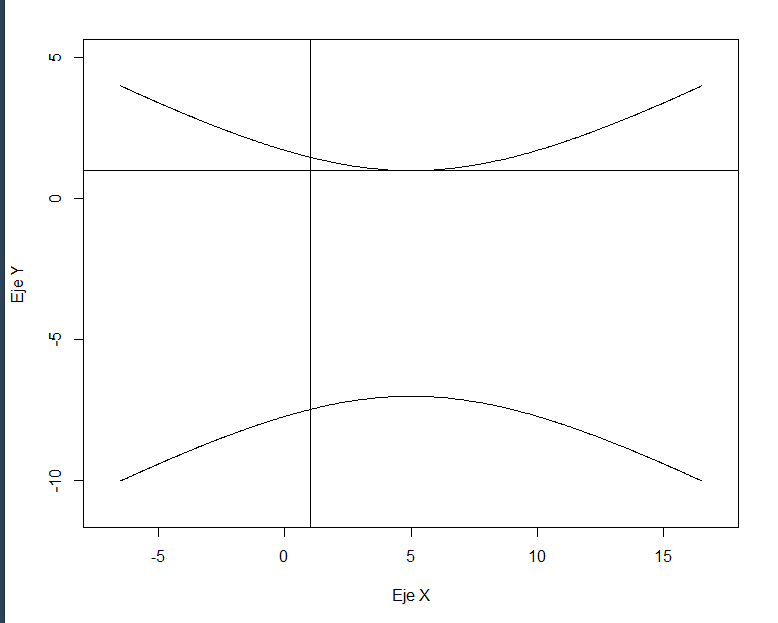
\includegraphics[width=10cm, height=5cm]{Grafica9}
    \caption{Gráfica de la hipérbola 1}
    \label{fig:mesh19}
\end{figure}

\textbf{Ejemplo 2:}

\begin{figure}[h]
    \centering
    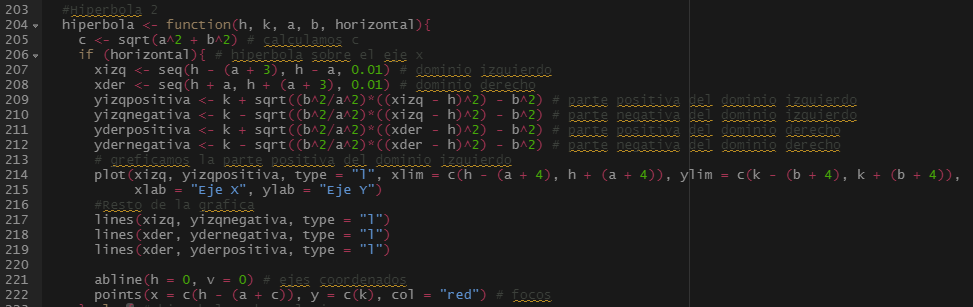
\includegraphics[width=12cm, height=5cm]{Codigohipe3}
    \caption{Código de la hipérbola 2 parte 1}
    \label{fig:mesh20}
\end{figure}

\newpage
\begin{figure}[h]
    \centering
    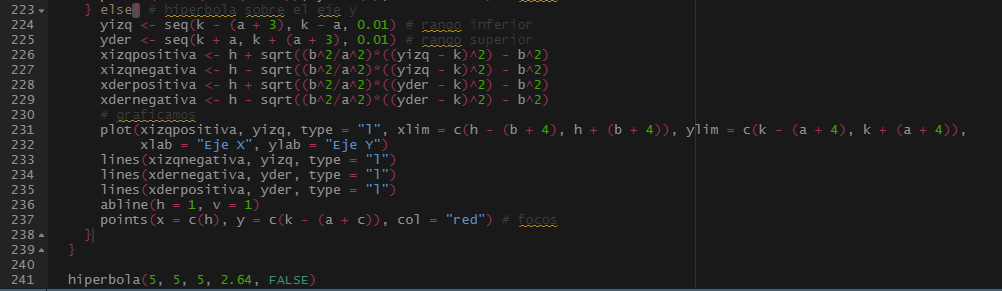
\includegraphics[width=12cm, height=5cm]{Codigohipe4}
    \caption{Código de la hipérbola 2 parte 2}
    \label{fig:mesh21}
\end{figure}
y su gráfica seria:
\begin{figure}[ht]
    \centering
    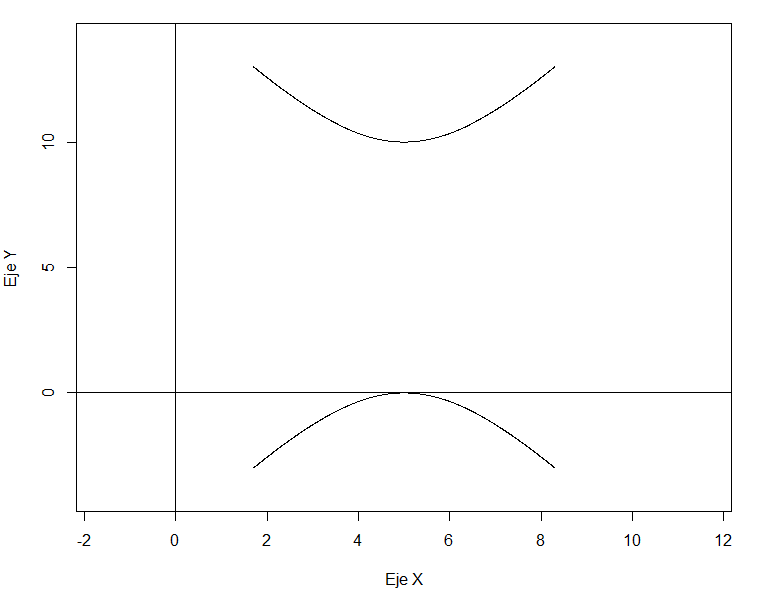
\includegraphics[width=10cm, height=5cm]{Grafica10}
    \caption{Gráfica de la hipérbola 2}
    \label{fig:mesh22}
\end{figure}



\begin{thebibliography}{0}
  \bibitem{Lemhann,1965} Charles H. Lemhann. Geometria Analitica, 1965.
  \bibitem{Jesus Rangel, Repositorio de GitHub}Jesus Rangel, repositorio de GitHub\textcolor{blue}{\url{https://github.com/JesusRangel07/MatematicasComputacionales}}\href{https://github.com/JesusRangel07/MatematicasComputacionales}{\textcolor{blue}{Repositorio de Github}}
\end{thebibliography}

\end{document}